

%ei varmaan saa olla kymy
\subsubsection{Mikä on React}

% https://github.com/facebook/react/blob/main/README.md
% https://www.infoq.com/news/2013/06/facebook-react/
% molemmat siteerattu 27.5.24


React on metan ylläpitämä avoimeen lähdekoodiin perustuva javascript kirjasto, joka on suunniteltu reaktiivisien käyttöliittyjien kehittämiseen.
%more text
%
Reaktia voi käyttää mobiili ja työpöytä sovelluksien käyttöliittymien kehittämiseen. 
\medskip




% https://react.dev/
% 30.5


%https://www.statista.com/statistics/1124699/worldwide-developer-survey-most-used-frameworks-web/
%yksi käytetyimmistä työkaluista 
% 30.5

%

React kannustaa kehittäjiä rakentamaan sovelluksia uudelleenkäytettävien komponenttien avulla.
Jokainen komponentti sisältää oman rakenteensa, tyylinsä ja käyttäytymisensä, joka tekee niistä helposti siirrettävän ja uudelleenkäytettävän.
Komponenteista voidaan sitten koota monimutkaisia käyttöliittymimä. 
Komponentit voidaan kirjoitetaa JSX syntaksilla, joka mahdollistaa HTML tyylisen kirjoituksen JavaScriptin sekaan.
Tämä tekee React:ista helppo ja luettavan, ymmärrettävän ja opittavan, joka on auttanut nostamaan reactin suosiota yhteen maailman käytetyimmistä käyttöliittymä työkaluista.
\medskip








\subsubsection{jsx}

%https://react.dev/learn/writing-markup-with-jsx
%https://facebook.github.io/jsx/ 

% jsx = js xml
% https://medium.com/@sjarancio/what-is-jsx-e3dda0af3490

%transpilation
%https://www.scholarhat.com/tutorial/react/getting-started-with-jsx
% https://www.typescriptlang.org/docs/handbook/jsx.html

% kaikki viitattu 27.5

%html koodia uusiks
JSX (javascript XML) on sytaksi jatke javascriptille, joka antaa kehittäjän kirjoittaa HTML tyylistä koodia javascriptin sekaan, tekien koodista yksinkertaisempaa ja helpompaa ymmärtää.
% suora sitaatti https://facebook.github.io/jsx/ 
JSX ei ole ECMAscript standardissa, joten selaimet eivät osaa tulkita sitä, vaan JSX se on suunniteltu transpiloitavaksi johonkin ECMAscript standardia toteuttavalle kielelle.
\medskip

\bigskip
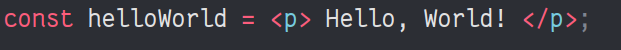
\includegraphics[width=10cm]{src/public/oppar/pure_jsx_example.png}

Kuva\getImgCount .{} kuvankaappaus JSX syntaxista.
\medskip

%muuttuja vois vaihtaa. johonkin toiseen suomalaiseen sanaan
Kuvassa luodaan muuttuja helloWorld, jolle annetaan arvoksi HTML "p"{} elementti, jossa teksti "Hello, World!"{}.
% koko juttu uusiks ja paremmin kirjoitettua
Muuttujien arvot voidaan kirjoittaa HTML tyylillä, tekien monimutkaisten elementtien rakentamisesta yksinkertaista.
\medskip



\bigskip
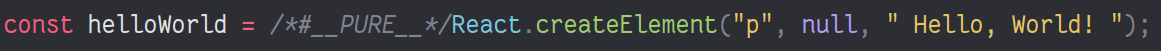
\includegraphics[width=15cm]{src/public/oppar/transpiled_jsx_example.png}

Kuva\getImgCount .{} Kuvankaappaus helloWorld muuttujasta, joka on transpiloitu javascriptiin. 
\medskip

%vähän toistoa muttei väliä sillä pitää siteerata tämä

%https://babeljs.io/repl 
Kuvassa on helloworld muuttuja, joka on käännetty natiiviksi javascriptiksi babel kääntäjää käyttäen.
Tämä antaa selaimille mahdollisuuden suorittaa koodia, joka on alkuperin kirjoitettu käyttämällä JSX syntaxia.
%jotain lisää
\medskip



\subsubsection{Komponentit}


% komponentti joka voi renderöidä toisen komponentin. tämä jatkuu siihen asti että päästään natiiveihin html elementteihin jotka selain osaa tulkita
%https://react.dev/learn/your-first-component

% mahdollisesti näytä ekaksi class componentti sitten funkitio komponentti.
% näin voi sitten jälkeempäin selittää mikä usestate hook on paremmin


React komponentti on oma kokoomus joka sisältää oman tilan, käyttäytymisen ja tyylin.

komponentti on oma pieni kokoompano joka sisältää sen ulkonäön ja käyttäytymisen. componentteja voidaan
\medskip
\bigskip

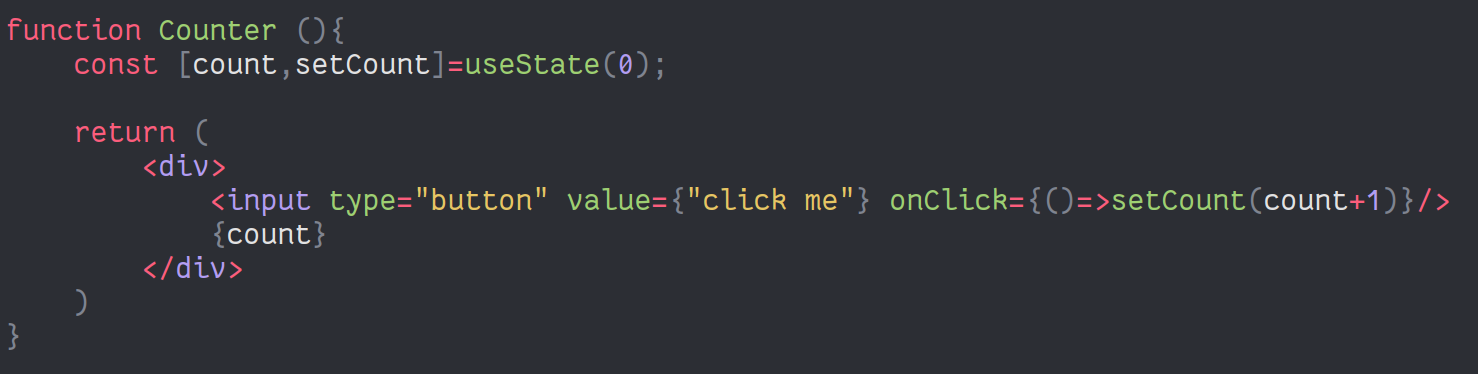
\includegraphics[width=15cm]{src/public/oppar/function_component.png}

Kuva \getImgCount{}. kuvakaappaus React komponentista
\medskip

kuvaassa teemmme funktio komponentin laskija joka seuraa kuinka monta kertaa nappia on painettu.
funktio palauttaa komponentin ulkonäön, joka on määritetty JSX syntaxilla.
komponentissa on myös useState "hook"{}, joka kuvaistaa komponentin tilan, tätä käytten komponentti pystyy säilyttämään dataa ja päivittämään itsensä kun sen sisäinen tila muuttuu.
\medskip

Komponentit voivat myös määrittää luokkakomponentti tyylillä. Mutta React on kehottaa käyttää funktio komponentteja tulevaisuudessa.
Kuva {\the\numexpr \theimgCounter + 1}{} on sama laskukomponentti kuin kuva \theimgCounter{} mutta kirjoitettu luokkakomponentti tyylillä. 
\medskip
\bigskip


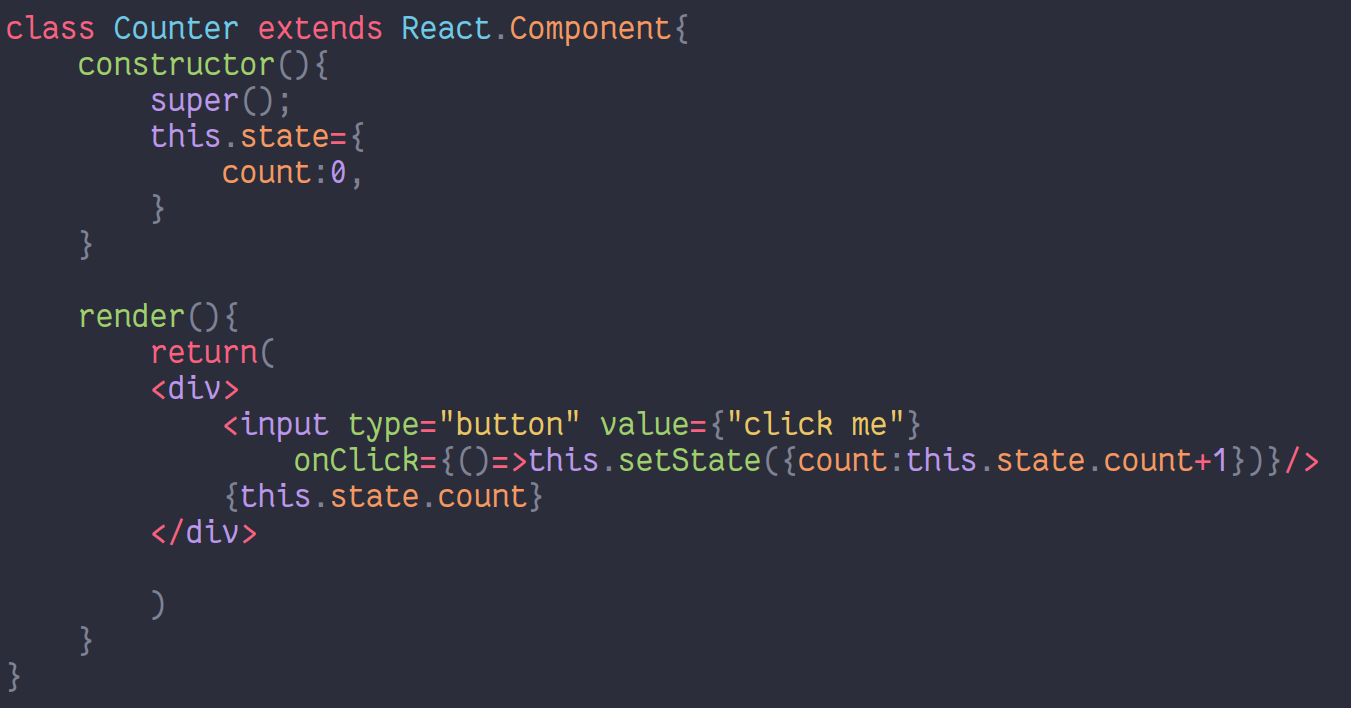
\includegraphics[width=15cm]{src/public/oppar/class_.png}

Kuva \getImgCount{}. kuvakaappaus React luokkakomponentista
\medskip

% get some src for this
% we can prob link the docs if we find the right page

Luokkakomponentissa komponentin tilaa säilytetään this.state ominaisuudessa, ja sitä voi muuttaa käyttämällä this.setState funktiolla. 
%ainakintoinen lauseke
\medskip

%https://react.dev/reference/react/hooks
% 31.5

Funktio componentissa tila hallinnoidaan "React hookeilla"{}. 
"Hookit"{} antavat funktio komponenteille mahdollisuuden käyttää Reactin ominaisuuksia, 
jotka luokkakomponentit saavat kun ne jatkavat React.Component luokkaa.
%
React kehottaa käyttämään funktiokomponentteja. ja niissä on myös vähemmän koodia kun luokka komponentissa vaikka lopputulos on sama.
Molemmat komponentit tehty react 18.3.1 versiolla.







\medskip

\subsubsection{Reaktin struktuuri ja toiminta}

% https://github.com/facebook/react/blob/a4195750779dbd9a13e1615fbbd493bf2c5768ca/packages/react/src/ReactElement.js#L362
%pitää vissii kysyy voiko lähdekoodia käyttää lähteenä..


%https://react.dev/reference/react-dom/client/createRoot
% viittaus 29.5

%laitetaanko kuva jostain indexistä
%vaikka joku joka on tehty create react app jutulla

jotain tekstiä reaktin toiminnasta 
\bigskip



Kuva \getImgCount{}. kuvankaappaus create-react-app komennon tekemästä index.js tiedostosta
\medskip

react tekee funktiolle antamasta elementistä Root elementin, ja se alkaa hallinnoimaan domia sen alla
\medskip

%jos nämä yhdistää tarvitaan toinen kappale. voitaisiin tosin kirjoittaa muutenkin toinen kappale toiminnasta. tai koko lifecyclestä
% ainakin jos mainitaan vdomista joitan

root.render
render funktio suorittaa komponentin funktiona. komponentti on jo tässä vaiheessa käännettu natiiviksi javascriptiksi, 
joten komponentin lapsikomponentit voidaan suorittaa samalla. Lopputuloksena saadaan natiivi html elementtejä jotka selain voi renderöidä.

\medskip



%joku maininta vdomista jossain vaiheessqa enne ntätä ja sitten siirrä oikeaan paikkaan
\subsubsection{DOM ja VDOM}


%jotain domista, mikä se on ja miten se liittyy käyttöliittymiin ja sitten mikä on vdom
% vai pitäisikö samantien aloittaa että meillä on vdom, ja sittem selittää mikä dom on..... kuulostaa väärältä

% https://www.w3.org/TR/WD-DOM/introduction.html
% 29.5


%psychotic
DOM (eng Document object model) on puu-struktuurinen representaatio HTML dokumentista.
Tätä struktuuria käytetään rajapintana JavaScriptin ja HTML:län välillä. 
Struktuurissa jokainen solmu on objekti, joka esittää osaa dokumentista. 
Soulmuissa voi olla yksi tai useampi objekti ja nämä objektit voivat osoittaa muihin solmuihin.



esimerkiksi dom representaatio seuraavasta html koodista

% https://www.w3.org/TR/WD-DOM/introduction.html
% kuva ja koodi molemmat täältä.. 29.5 viitatti
    
%pitää viitata jotenkin
\begin{tcolorbox}
\begin{lstlisting}[language=html]
<TABLE>
    <ROWS> 
      <TR> 
          <TD>Shady Grove</TD>
          <TD>Aeolian</TD> 
      </TR> 
      <TR>
          <TD>Over the River, Charlie</TD>
          <TD>Dorian</TD> 
      </TR> 
    </ROWS>
</TABLE>
\end{lstlisting}
\end{tcolorbox}


Esimerkki HTML koodissa luomme pöydän, jossa tehdään kaksi riviä ROWS elementin alle. 
%sisältää väärä sana
Joka riviin tulee kaksi "table data"{} elementtiä, jotka sisältää datan tekstinä.
\bigskip



%kuva html domista
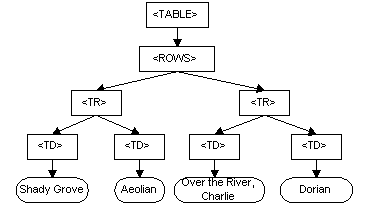
\includegraphics{./src/public/oppar/dom.png}

Kuva\getImgCount .{} DOM puu esimerkki HTML koodista. Jonathan Robie, Texcel Research 
\medskip

Kuvassa on esimerkki HTML koodista tehty DOM puu struktuuri.
tätä käyttämällä, 

jotain rajapinta interaktiivisuus helppokäyttöisyys javascript jne lorem ipsum lorem ipsumlorem ipsumlorem ipsumlorem ipsum

\bigskip



%https://medium.com/@BharathkumarV/reacts-virtual-dom-17fdcb290a10
% siteerattu 27.5

VDOM (eng Virtual Dom) on virtuaalinen esitys DOM:ista, jonka react pitää musitissaan koko suorituksen ajan.
VDOM:ia käyttäen react voi nopeasti päätellä mitkä osat käyttöliittymästä pitää päivittää, kun jonkun komponentin tila päivittyy. 
\medskip



